\documentclass[tikz,border=8pt]{standalone}
\usepackage{amsmath,amssymb}
\usepackage{xcolor}

\definecolor{navyblue}{RGB}{0,32,96}
\definecolor{tealblue}{RGB}{0,128,128}
\definecolor{crimsonred}{RGB}{192,41,43}
\definecolor{slatebg}{RGB}{245,247,250}

\usetikzlibrary{arrows.meta,calc,decorations.markings,shadows.blur}

\begin{document}
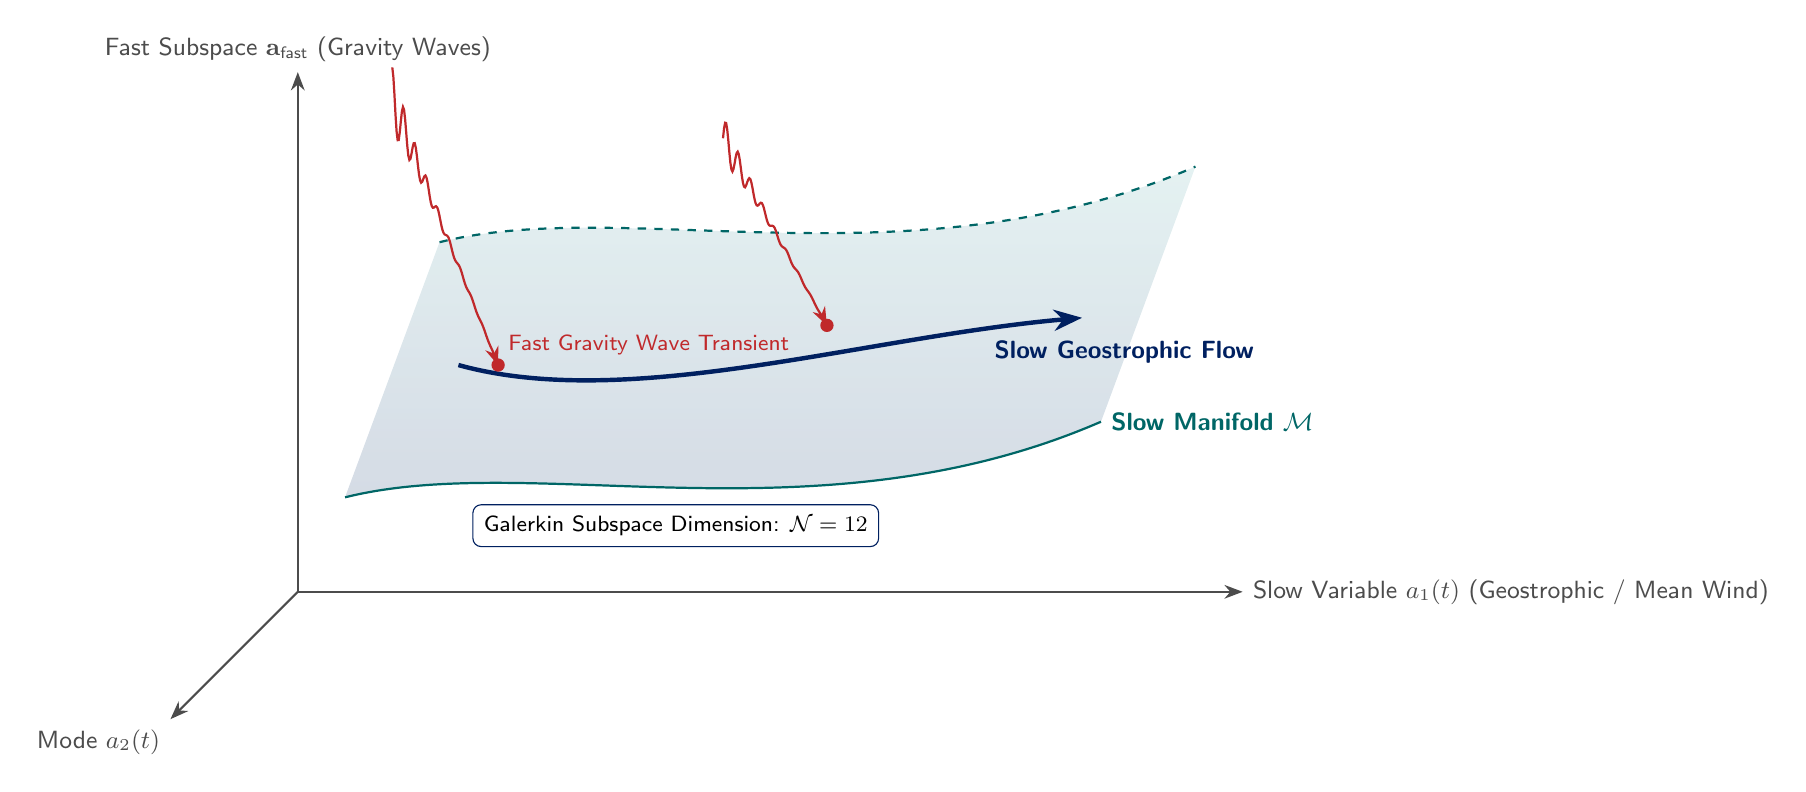
\begin{tikzpicture}[
    scale=1.2,
    >=Stealth,
    axis/.style={->, thick, color=black!70},
    fasttrajs/.style={crimsonred, thick, ->},
    slowtraj/.style={navyblue, ultra thick, ->}
]

    % Draw manifold surface background
    \shade[top color=tealblue!15, bottom color=navyblue!25, opacity=0.7]
        (0,0) .. controls (2,0.5) and (5,-0.5) .. (8,0.8)
        -- (9,3.5) .. controls (6,2.2) and (3,3.2) .. (1,2.7) -- cycle;

    % Manifold Boundary Frame
    \draw[tealblue!80!black, thick]
        (0,0) .. controls (2,0.5) and (5,-0.5) .. (8,0.8)
        node[right, font=\small\sffamily\bfseries] {Slow Manifold $\mathcal{M}$};
    \draw[tealblue!80!black, thick, dashed]
        (1,2.7) .. controls (3,3.2) and (6,2.2) .. (9,3.5);

    % Coordinate Axes (Fast Modes vs Slow Variables)
    \draw[axis] (-0.5,-1,0) -- (9.5,-1,0) node[right, font=\small\sffamily] {Slow Variable $a_1(t)$ (Geostrophic / Mean Wind)};
    \draw[axis] (-0.5,-1,0) -- (-0.5,4.5,0) node[above, font=\small\sffamily] {Fast Subspace $\mathbf{a}_{\text{fast}}$ (Gravity Waves)};
    \draw[axis] (-0.5,-1,0) -- (-0.5,-1,3.5) node[below left, font=\small\sffamily] {Mode $a_2(t)$};

    % Slow Manifold Trajectory
    \draw[slowtraj] (1.2, 1.4) .. controls (3.0, 0.9) and (5.5, 1.7) .. (7.8, 1.9)
        node[pos=0.85, below right, font=\small\sffamily\bfseries, color=navyblue] {Slow Geostrophic Flow};

    % Fast Oscillatory Decay Trajectories (Collapsing onto Slow Manifold)
    % Trajectory 1
    \draw[fasttrajs, domain=0:2.8, samples=100, variable=\t]
        plot ({0.5 + 0.4*\t}, {4.2 - 1.0*\t + 0.35*exp(-1.5*\t)*cos(1200*\t)})
        node[above right, font=\footnotesize\sffamily, color=crimsonred] {Fast Gravity Wave Transient};

    % Trajectory 2
    \draw[fasttrajs, domain=0:2.2, samples=100, variable=\t]
        plot ({4.0 + 0.5*\t}, {3.8 - 0.9*\t + 0.25*exp(-1.8*\t)*sin(1400*\t)});

    % Impact Points on Manifold
    \fill[crimsonred] (1.62, 1.4) circle (2pt);
    \fill[crimsonred] (5.10, 1.82) circle (2pt);

    % Labels and Annotations
    \node[draw=navyblue, fill=white, rounded corners=3pt, inner sep=4pt, font=\footnotesize\sffamily]
        at (3.5, -0.3) {Galerkin Subspace Dimension: $\mathcal{N}=12$};

\end{tikzpicture}
\end{document}